\chapter{Introduction and Literature Review}

Glaucoma is a group of progressive optic neuropathies where vision loss results from slow progressive degeneration of retinal ganglion cells and their axons. \cite{Weinreb2004} Patients are typically elderly. The loss of vision is irreversible. As a result, it is a leading cause of blindness worldwide. 

If glaucoma is detected and monitored in its early stages, it is treatable and can be reasonably well managed. This detection and monitoring relies upon imaging, and psycho-physical tests. A typical procedure includes examination of the optic disk, \ac{RNFL} with \ac{OCT}, measurement of \ac{IOP}, and \ac{VF} test.

Currently, the pathophysiology of glaucoma is not well understood and there are no models that can robustly characterize glaucoma progression \cite{Chen2014}. Glaucoma treatment relies heavily on accurate and timely prediction of the progress of the disease where patients with slowly progressing glaucoma might only require active surveillance, while fast progressors would require immediate intervention. Since glaucoma can eventually cause blindness, an accurate prediction of the progress of the disease will support optimal treatment decisions that are critical for the patient’s quality of life.  

\section{Background: Visual Field Test}

\ac{VF} testing is the current gold standard in clinical functional evaluation of glaucoma patients. It is used to both diagnose glaucoma, and in patients with confirmed or suspected glaucoma, to monitor the progression of the disease. Global VF indices such as \ac{MD} (also known as Mean Deviation Index), \ac{PSD}, and \ac{VFI} (also known as Glaucoma Progression Index) are used to monitor the integrity of the VF. These indices characterize each visual field with few statistical measures that attempt to capture the relevant clinical information to diagnose glaucoma and determine the progression of the disease. 

\begin{figure}[t]
	\centering
	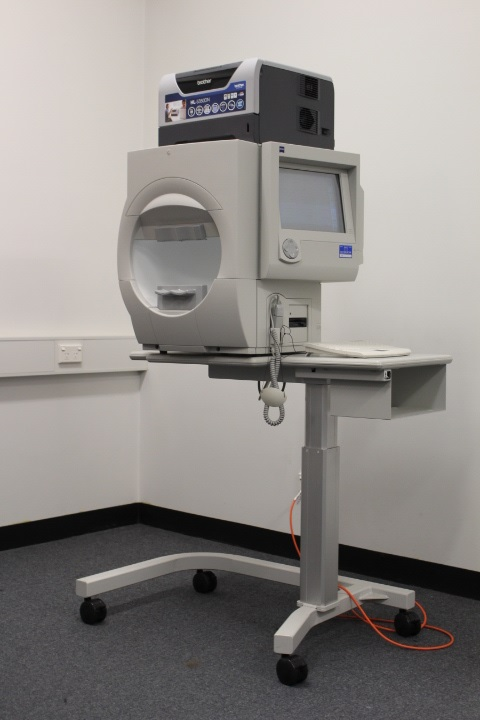
\includegraphics[width=0.5\textwidth]{hfa}
	\caption{An \ac{HFA} (``Humphrey VF'' by Sej licensed under \href{https://creativecommons.org/licenses/by-sa/4.0/deed.en}{CC BY-SA 4.0})}
	\label{fig:hfa}
\end{figure} 

\begin{figure}[p]
	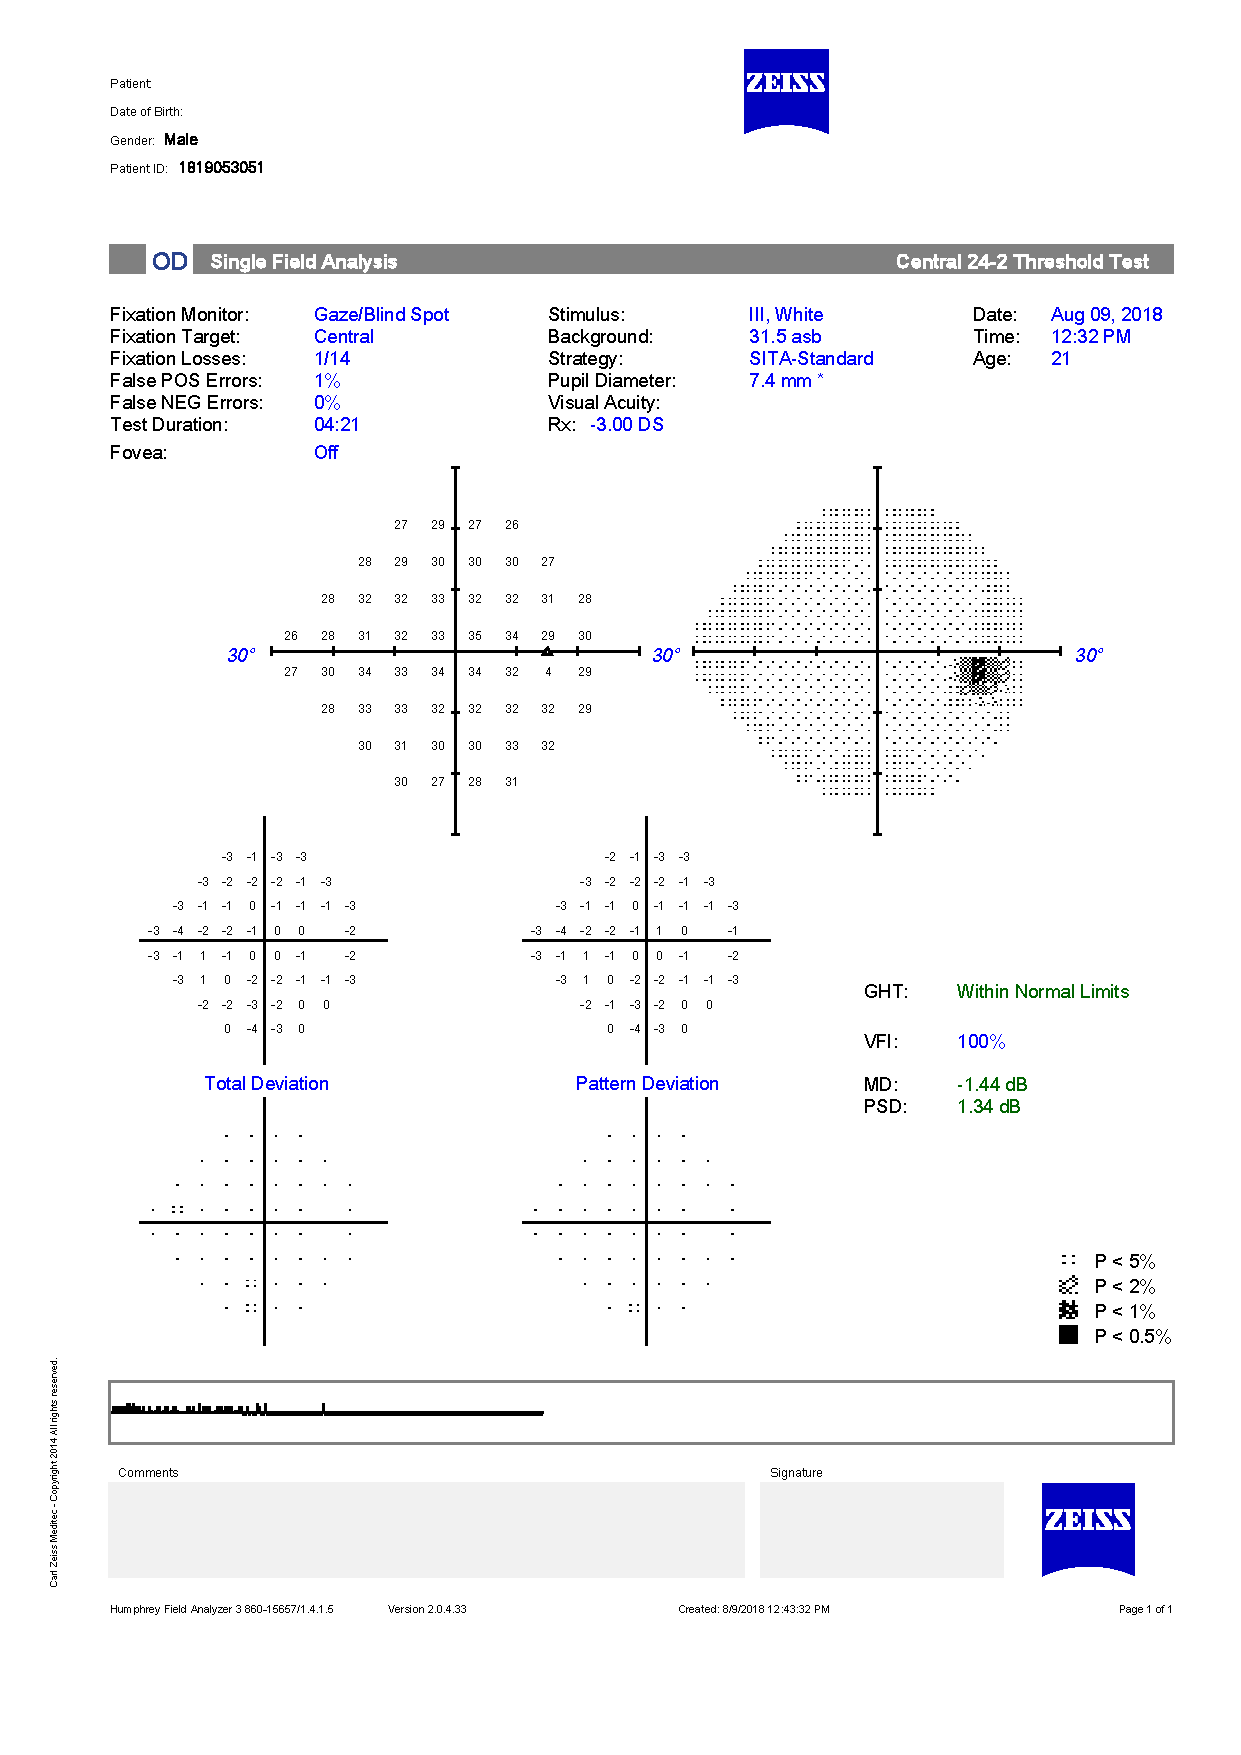
\includegraphics[width=0.9\textwidth]{report}
	\caption{Example of an \ac{HFA} \ac{VF} test report}
	\label{fig:report}
\end{figure}

\begin{figure}[p]
	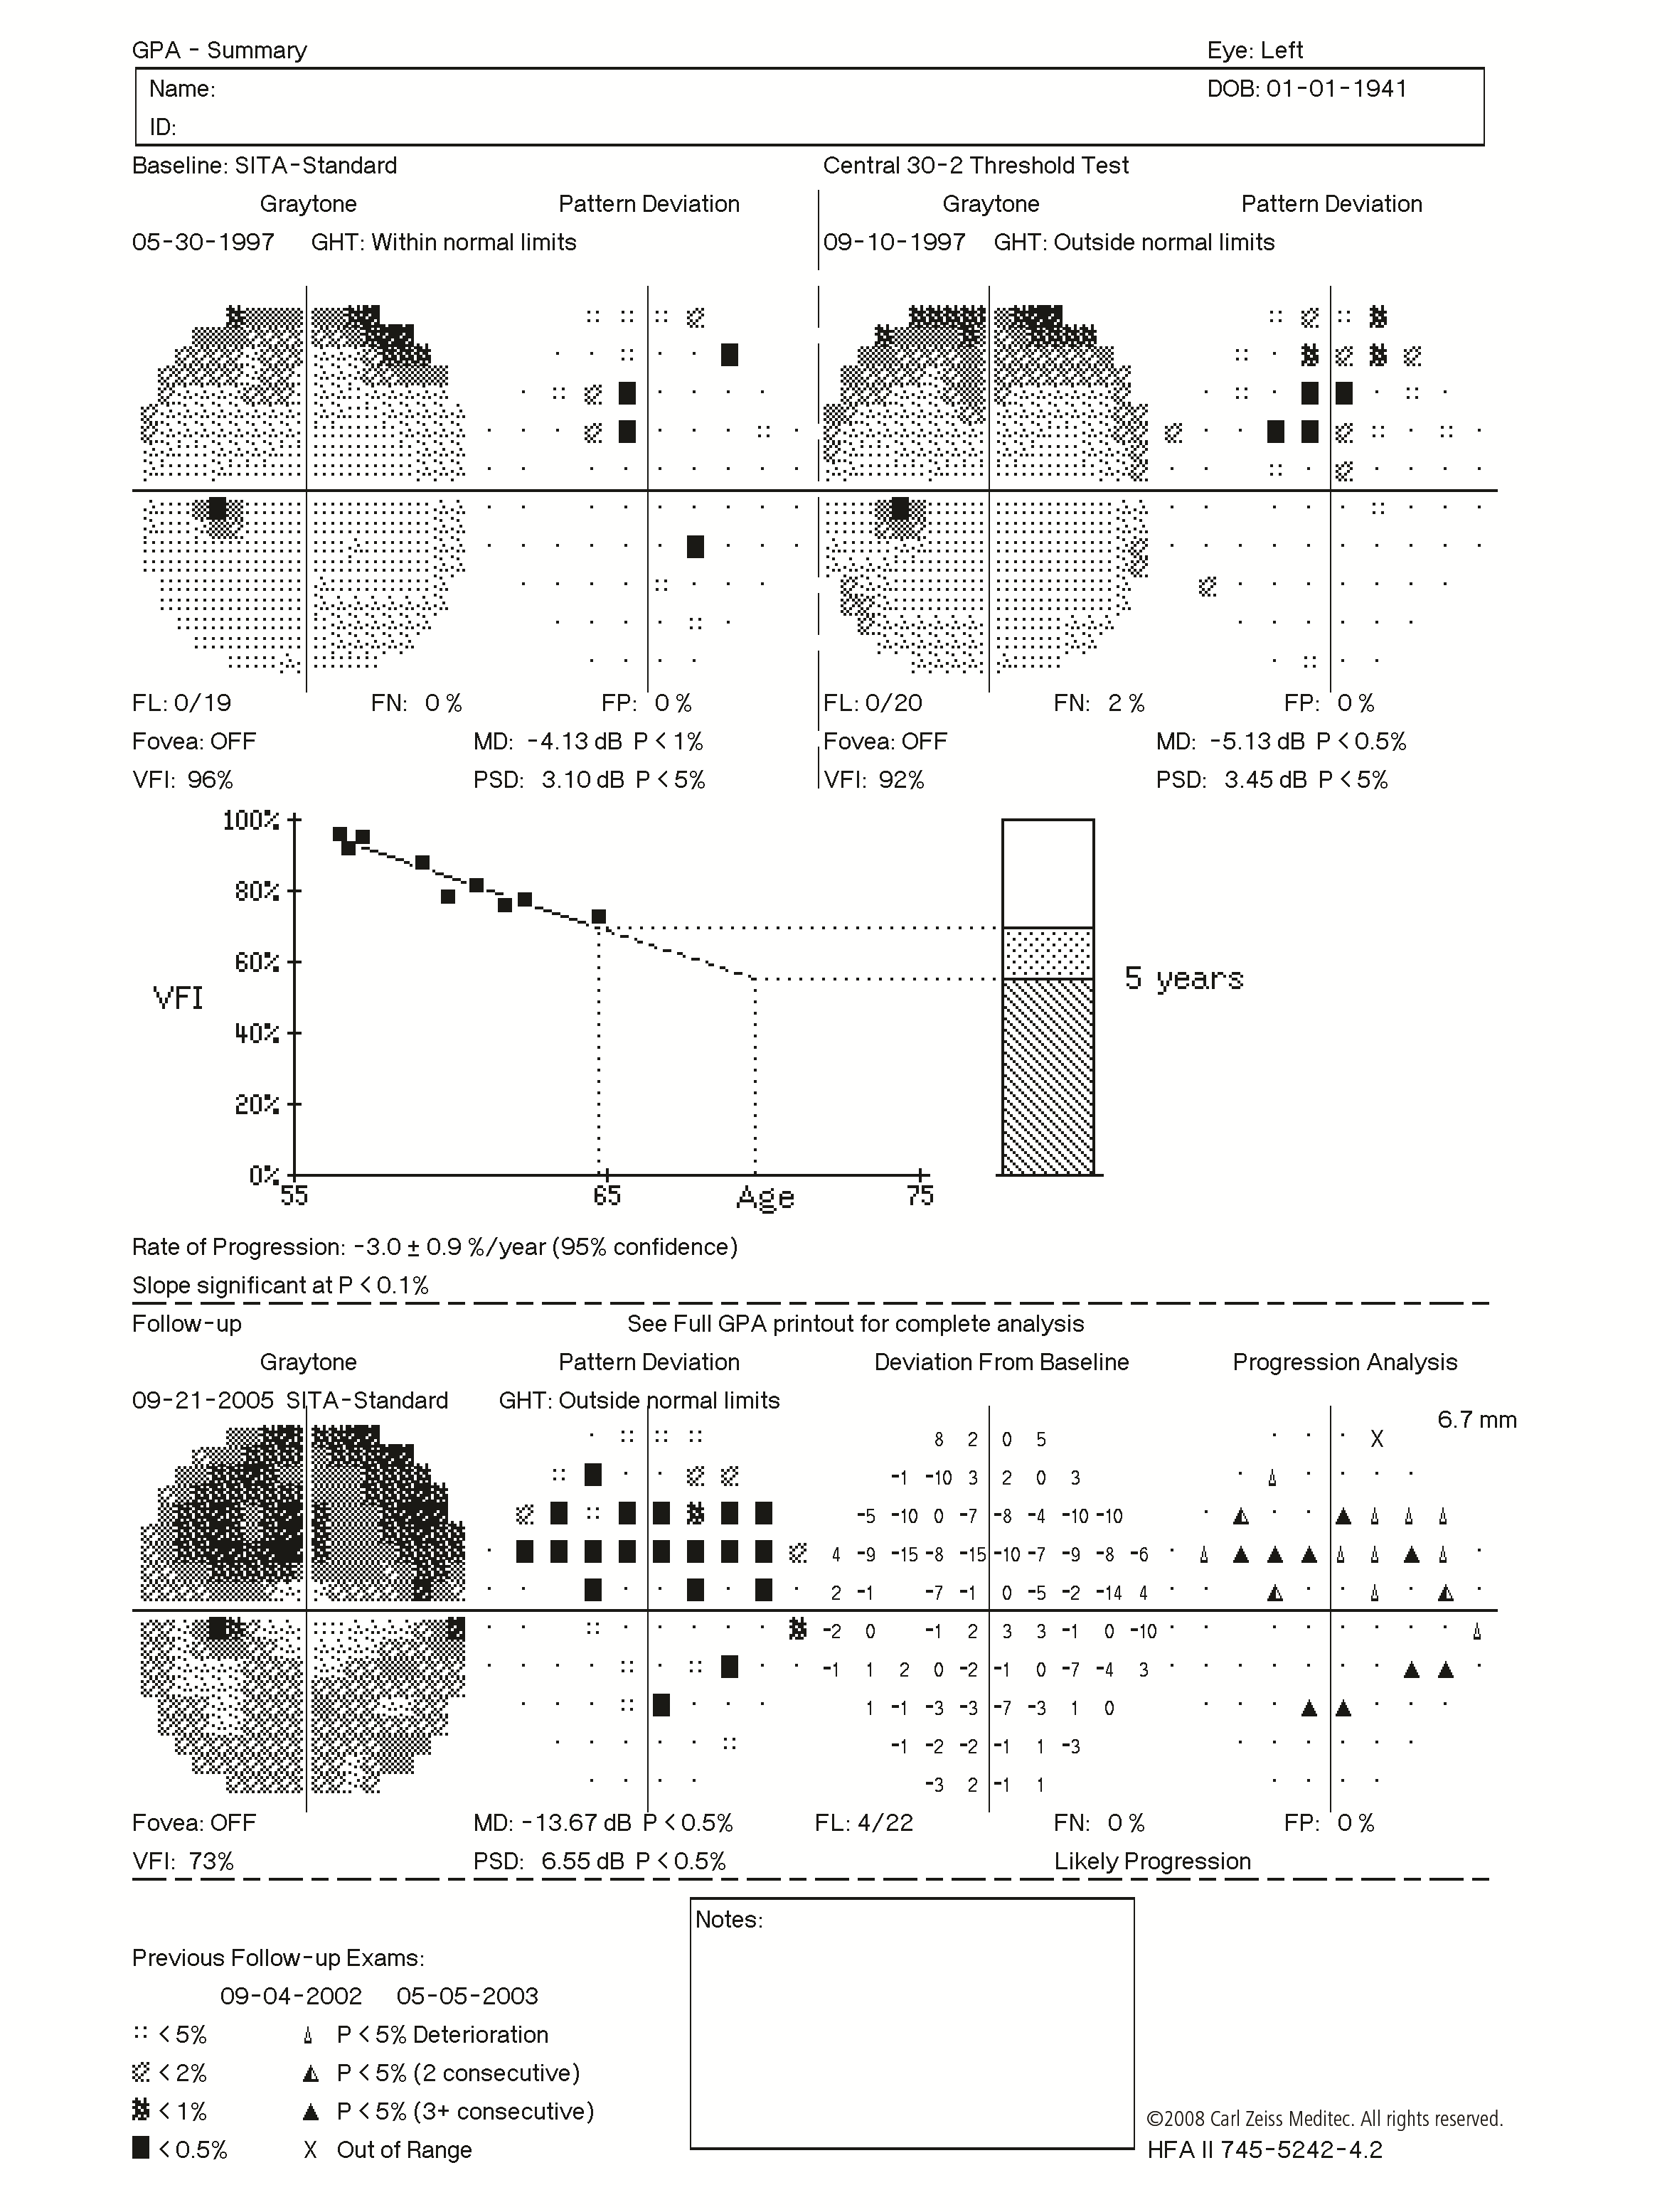
\includegraphics[width=\textwidth]{gpa}
	\caption{Example of an \ac{HFA} progression analysis test report (Image from Carl Zeiss Meditec, Inc.)}
	\label{fig:gpa}
\end{figure}

\subsection{Single Field Analysis Metrics}

Historically Heijl et al. developed the two classic metrics for summarizing a \ac{VF}: \ac{MD} and \ac{PSD}. \cite{Heijl1987} First and foremost, to evaluate one's visual field, it is necessary to know the appropriate reference threshold ($N$) at each field location with an associated variance ($\sigma^2$). It is widely accepted that the human \ac{DLS} thresholds, in units of dB, can be modeled as a linear function of age. \cite{Heijl1987a} In general, the slope of loss of sensitivity is larger in mid-periphery than para-centrally, range from $0.5$ to $1$ dB/decade. The variance is also higher in mid-periphery than para-centrally. 

\ac{MD} is a measure of a \ac{VF}'s general mean value as compared to the reference. Mathematically, it is the mean of the difference between the measured threshold ($x$) and the reference $N$, weighted by the variance. Points with higher variance are considered less reliable and given less weight in the \ac{MD} metric; blind spots (i.e. ($15\degree$, $\pm3\degree$) are removed). MD values typically range from negative to slightly positive. Negative MD values indicate less than normal sensitivity in the entire \ac{VF} and the patient may be suspected of glaucoma and/or cataract.

\begin{equation} \label{eq:md}
\textrm{MD} =\frac{ 
\sum\limits_{i=1}^{n} \left\{
\frac{1}{\sigma_{i}^2} (x_i-N_i)
\right\} }{
\sum\limits_{i=1}^{n} 
\frac{1}{\sigma_{i}^2} 
}
\end{equation}

While the \ac{MD} is an intuitive summary metric for a \ac{VF}, it captures the general reduction in sensitivity, which is typical of cataract, but does not capture local asymmetries (variations) in the field, which is typical in a glaucomatous field. \ac{PSD} is another metric that tries to capture this asymmetry. Mathematically, it is defined as the weighted variance of the field, as defined in \cref{eq:psd}. $n$ refers to the numbers of locations, less the two blind spots, in the test pattern used for calculation (e.g. $n=54-2$ for the 24-2 pattern). \ac{PSD} is always positive, with higher value indicating a more varying field with a higher likelihood of glaucoma.

\begin{equation} \label{eq:psd}
\textrm{PSD}^2 =
	\frac{1}{n}
	\sum\limits_{i=1}^{n} 
	\sigma_{i}^2
	\times
	\frac{1}{n-1}
	\sum\limits_{i=1}^{n} 
	\frac{(x_i-N_i-\textrm{MD})^2}{\sigma_{i}^2} 
\end{equation}

Recently the new \ac{VFI} metric has become available on \ac{HFA} field analysis reports. It attempts to reduce the influence of cataract on \ac{MD} and is argued to be a better indicator for glaucoma doctors. It is reported as a percentage with $100\%$ being a perfectly healthy field and $0\%$ being a blind field. \cite{Bengtsson2008}

Another metric developed is \ac{GHT}. It combines measurement of the overall field sensitivity and differences between the top and half hemi-fields into a few hand-crafted ``if'' statements to report a field as one of the following categories for easy interpretation: \cite{Asman1992}

\begin{itemize}
	\item Abnormally high sensitivity
	\item Outside normal limits
	\item Borderline
	\item General reduction of sensitivity
	\item Within normal limits
\end{itemize}

These four metrics can be seen in figure \ref{fig:report}.

\subsection{Trend-Based Progression Analysis}

Currently, the main approach to determine glaucoma progression is a trend-based analysis by performing \ac{OLSLR} on MD. The \ac{HFA} Guided Progression Analysis reports \ac{OLSLR} on its \ac{VFI} that offers similar information. The fitted trend is typically extended five years into the future, and the slope of the line is used to classify patients into three categories (mild: $0$ to $-0.4$ dB/year, moderate: $-0.5$ to $-2$ dB/year, and severe: $<-2$ dB/year). \cite{Chauhan2008} Glaucoma specialists combine these data with additional information such as the thickness of the retinal fiber layer in the macula, \ac{IOP} and the cup-to-disk ratio to determine the optimal plan of treatment. 

\subsection{Limitations}

The current method of evaluating \ac{VF} information is limited in its robustness. For example, \ac{VFI} may remain at $100\%$ in $22\%$ patients who have MD of $-5$ dB or better. Hence early progression (up to $-5$ dB) may be missed if VFI alone is used. Moreover, based on a semi-annual follow-up schedule, at least five fields are required to produce an accurate prediction for a disease that is progressing at moderate rates (the slope of the OLSLR on MD is $-1.0$ dB/year). \cite{Chauhan2008} This means that meaningful decision about the progression of the disease cannot be made until at least two years after the initial visit. 

Last but not least, \ac{OLSLR} is a simple model chosen based on its mathematical simplicity but not upon physiology. Since glaucoma can be caused by multiple neurological pathways, it is argued that the progression trend is likely nonlinear in nature. \cite{Pathak2013} 

In short, the use of linear regression to predict \ac{VF} loss and the need for a long observation period impede timely and accurate decision making by the clinician. A better method that can provide more accurate information to the clinician in fewer \ac{VF} tests can allow more effective intervention for glaucoma patients in the disease's early stages. This is the primary motivation for the alternative models reviewed below and for the current work.

\section{Literature Review: Alternative Progression Models}

This section will review alternatives to the \ac{OLSLR} on MD model for \ac{VF} progression prediction. 

\subsection{Statistical Models}

A complement to trend-based analysis is event-based analysis. A popular implementation is the Glaucoma Progression Analysis (GPA) since it is provided by the \ac{HFA}. Instead of fitting a trend on a global index, the progression of each point in the field with respect to a baseline measurement is considered. On average, this method is found to have low false-positive rate. However, this is dependent upon achieving a good baseline and does not work for patients with severe \ac{VF} loss. \cite{Aref2017}

Other non-linear models suggest fitting an exponential model to the \ac{VF} indices. For example, Pathak et al. argued that an exponential model is better supported by recent knowledge of structure-function relationship than a linear model. \cite{Pathak2013} They demonstrated that a linear mixed-effect (LME) approach with an exponential model provided significantly better prediction of glaucoma progression than linear models. However, it is also pointed out that even though the LME approach has better results than the \ac{OLSLR} it still cannot capture the full extent of glaucomatous \ac{VF} change.

Other innovative approaches to the glaucoma progression problem in the literature include:

\begin{itemize}
	\item Point-wise linear regression (PLR): Developed for improving early detection, PLR combines event-based and trend-based analysis \cite{Nouri-Mahdavi2005}. 
	\item Analysis with Non-Stationary Weibull Error Regression and Spatial Enhancement (ANSWERS): Using spatial correlation between points and incorporating non-stationary variability; progression detection was found to be better especially in short time series \cite{Zhu2015}.
	\item Spatially filtering \ac{VF} data before PLR analysis: By applying a spatial filter that incorporates physiological relationships between measured contrast sensitivities at test points within the VF, the specificity of the PLR method is not affected but the sensitivity of detecting the rate of progression is improved \cite{Strouthidis}.
\end{itemize}

\subsection{Machine Learning Models}

The above methods use different approaches to improve the prediction of glaucoma progression and demonstrate the complexity of the prediction task. This is not surprising due to the complex nature of the disease. A natural step forward involves leveraging the power of modern \ac{ML} techniques to integrate features such as non-linear trends, correlation between \ac{VF} test locations, field patterns, etc. into a single model.
 
Existing studies have demonstrated the usefulness of \ac{ML} in glaucoma care. For example, Asaoka et al. compared the performance of traditional ML classifiers with that of a deep feed-forward neural network (FNN) in diagnosing preperimetric glaucoma with VF data \cite{Asaoka2016}. Their FNN model performed significantly better than other methods. In another study, Yousefi et al. applied clustering algorithms to extract VF patterns as features, then adapted the traditional linear regression algorithm to model the features to generate the predictions \cite{Yousefi2018}. The \ac{ML}-based index for the detection of glaucoma progression outperformed current methods. 

However, these studies either did not directly address the problem of predicting \ac{VF} progression or only used traditional \ac{ML} methods for initial feature extraction. In a recent study that fully utilized the power of \ac{ML} for the prediction task, Wen et al. \cite{Wen2018} used deep learning network to predict future VF given the measurements of a single current \ac{VF}. Their deep learning network demonstrated amazing capability to generate prediction for future VFs for up to $5.5$ years with a correlation of $0.92$ between the predicted \ac{MD} and actual future \ac{MD} (average difference of $0.41$ dB). Their results suggest the tremendous potential of this research area. 

Another benefit of using an \ac{ML} model is the ability to use VF data (i.e. functional indication of \ac{VF} integrity) and \ac{OCT} data (i.e. structural indication for the integrity of the retina) at the same time. It is known that by utilizing both \ac{VF} and \ac{OCT} data the sensitivity of glaucoma detection can be improved \cite{Shah2006}, \cite{Lu2008}. Multivariate models including both \ac{VF} and \ac{OCT} have also been shown to be successful \cite{Mwanza2013}. However, there is limited research on combining \ac{VF} and \ac{OCT} features through a \ac{ML} model. A limited attempt to explore this idea by Silva et al. did not produce better results than those obtained by \ac{VF} only parameters \cite{Silva2013}. 

In our study we plan to use \ac{ML} models that combine \ac{VF} and \ac{OCT} data for prediction of disease progression.  Specifically, we will use a deep \ac{RL} approach to the glaucoma progression problem. Deep RL has gained attention lately due to its use in solving seemingly impossible problems. The most well-known example is solving the ancient Go game, which is considered to be orders of magnitude more difficult than chess and other board games \cite{Silver2016}. \ac{RL} has also been used in the context of healthcare for discovering optimal, individualized treatment strategies for lung cancer \cite{Zhao2009}\cite{Zhao2011}, HIV \cite{Ernst2006} and neurological disorders \cite{Shortreed2011}. To the best of our knowledge this will be the first study to use \ac{RL} to predict glaucoma progression. 

